\everymath{\displaystyle}
\documentclass{beamer}
% \documentclass[handout]{beamer}

%\usepackage[pdftex]{color,graphicx}
\usepackage{amsmath,amssymb,amsfonts}

\mode<presentation>
{
  % \usetheme{Darmstadt}
  % \usetheme[hideothersubsections]{Hannover}
  % \usetheme[hideothersubsections]{Goettingen}
  \usetheme[hideothersubsections, right]{Berkeley}

  \usecolortheme{seahorse}
  % \usecolortheme{dolphin}
  \usecolortheme{rose}
  % \usecolortheme{orchid}

  \useinnertheme[shadow]{rounded}

  \setbeamercovered{transparent}
  % or whatever (possibly just delete it)
}

\mode<handout>{
  \setbeamercolor{background canvas}{bg=black!5}
  \usepackage{pgfpages}
  \pgfpagesuselayout{4 on 1}[a4paper,border shrink=5mm, landscape]
}

\usepackage[brazilian]{babel}
% or whatever

% \usepackage[latin1]{inputenc}
\usepackage[utf8]{inputenc}
% or whatever

\usepackage{times}
%\usepackage[T1]{fontenc}
% Or whatever. Note that the encoding and the font should match. If T1
% does not look nice, try deleting the line with the fontenc.


\title%[] % (optional, use only with long paper titles)
{Estrutura do trabalho acadêmico I}

\subtitle
{Conteúdos das seções} % (optional)

\author%[] % (optional, use only with lots of authors)
{Felipe Figueiredo}% \and S.~Another\inst{2}}
% - Use the \inst{?} command only if the authors have different
%   affiliation.

\institute[INTO] % (optional, but mostly needed)
{Instituto Nacional de Traumatologia e Ortopedia
}
  % \inst{1}%
  % Department of Computer Science\\
  % University of Somewhere
  % \and
  % \inst{2}%
  % Department of Theoretical Philosophy\\
  % University of Elsewhere}
% - Use the \inst command only if there are several affiliations.
% - Keep it simple, no one is interested in your street address.

\date%[] % (optional)
{}

% \subject{Talks}
% This is only inserted into the PDF information catalog. Can be left
% out. 



% If you have a file called "university-logo-filename.xxx", where xxx
% is a graphic format that can be processed by latex or pdflatex,
% resp., then you can add a logo as follows:

\pgfdeclareimage[height=1.6cm]{university-logo}{../logo}
\logo{\pgfuseimage{university-logo}}



% Delete this, if you do not want the table of contents to pop up at
% the beginning of each subsection:
\AtBeginSubsection[]
%\AtBeginSection[]
{
  \begin{frame}<beamer>{Sumário}
    \tableofcontents[currentsection,currentsubsection]
  \end{frame}
}


% If you wish to uncover everything in a step-wise fashion, uncomment
% the following command: 

% \beamerdefaultoverlayspecification{<+->}


\begin{document}

\begin{frame}
  \titlepage
\end{frame}

\begin{frame}{Sumário}
  \tableofcontents
  % You might wish to add the option [pausesections]
\end{frame}


%% Template
% \section{}

% \subsection{}

% \begin{frame}{}
%   \begin{itemize}
%   \item 
%   \end{itemize}
% \end{frame}

% \begin{frame}
%   \begin{columns}
%     \begin{column}{5cm}
%     \end{column}
%     \begin{column}{5cm}
%     \end{column}
%   \end{columns}
% \end{frame}

% \begin{frame}{}
%   \includegraphics[height=0.4\textheight]{file1}
%   \includegraphics[height=0.4\textheight]{file2}
%   \includegraphics[height=0.4\textheight]{file3}
%   \begin{figure}
%     \caption{}
%   \end{figure}
% \end{frame}

% \begin{frame}{}
%   \begin{definition}
%   \end{definition}
%   \begin{example}
%   \end{example}
%   \begin{block}{Exercício}
%   \end{block}
% \end{frame}

\section{Discussão da aula passada}

% \subsection{Discussão da aula passada}

\begin{frame}{Discussão da aula passada}
  \begin{block}{}
    Discussão da leitura obrigatória da aula passada
  \end{block}
\end{frame}

\section{Seções do Trabalho Acadêmico}

% \subsection{O Projeto}

\begin{frame}
  \begin{center}
    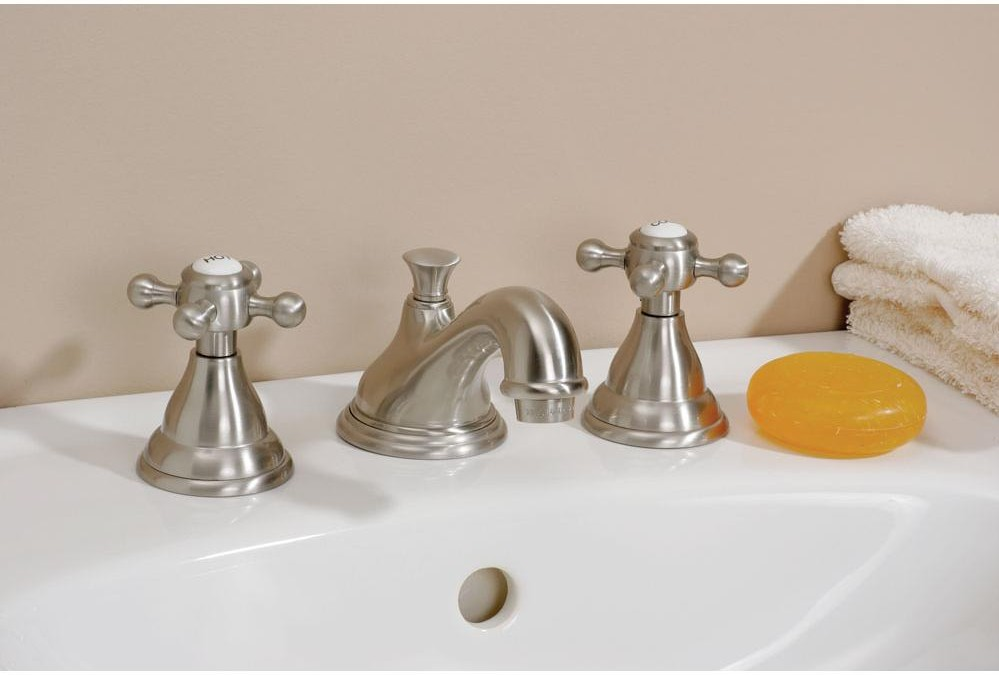
\includegraphics[height=.8\textheight]{EstruturaI/torneira}

    \visible<1>{Para que duas torneiras em uma bica?}

    \visible<2>{Qual é a quente e a qual é a fria?}
  \end{center}
\end{frame}

\begin{frame}{De que lado você sobe? Por que?}
  \begin{center}
    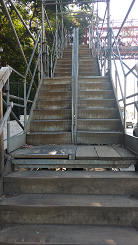
\includegraphics[height=\textheight]{EstruturaI/escada}
  \end{center}
\end{frame}

% \begin{frame}{O projeto}
%   \begin{itemize}
%   \item Delineia um \alert{plano} de pesquisa
%   \item Descreve a justificativa e motivação da pesquisa
%   \item Indica os métodos propostos e resultados esperados
%   \item Mostra resultados preliminares (caso disponíveis)
%   \item Tempo verbal usado: \alert{futuro} (ex: faremos, estudaremos,
%     analisaremos\ldots)
%   \end{itemize}
% \end{frame}

% \begin{frame}
%   \begin{block}{Projeto}
%     O texto do projeto deve detalhar (para o leitor) como se processará
%     todo o trabalho de pesquisa.
%   \end{block}
% \end{frame}

\subsection{Estrutura do trabalho}

\begin{frame}{Estrutura típica de um trabalho}
  \begin{enumerate}
    \footnotesize
  \item Páginas pré-textuais
    \begin{itemize}
      \scriptsize
    \item<2,6> Título \visible<6->{(\alert{{\bf o quê?}})}
    \item<2> Capa (Autores, etc...)
    \item<2> Sumários e listas
    \item<2> etc...
    \end{itemize}
  \item Introdução \visible<6->{(\alert{{\bf por quê?}})}
    \begin{itemize}
      \scriptsize
    \item<3> Contexto
    \item<3> Justificativa (ou Motivação)
    \item<3> Revisão bibliográfica\footnote{\tiny por vezes chamado
        de Fundamentação Teórica}
    \item<3,6> Objetivos \visible<6->{(\alert{{\bf para quê?}})}
    \end{itemize}
  \item Desenvolvimento
    \begin{itemize}
      \scriptsize
    \item<4,6> Metodologia ou Materiais e Métodos \visible<6->{(\alert{{\bf como?}})}
    \item<4> Resultados (relatório)
    \end{itemize}
  \item Encerramento
    \begin{itemize}
      \scriptsize
    \item<5,6> Cronograma (projeto) \visible<6->{(\alert{{\bf quando?}})}
    \item<5> Conclusão (relatório)
    \item<5> Referências
    \end{itemize}
  \end{enumerate}

  \vfill
  \scriptsize
  Esta é a ordem em que os conteúdos são apresentados ao leitor.
\end{frame}

% \begin{frame}{Estrutura típica de um trabalho}
%   \begin{itemize}
%     \footnotesize
%   \item<1-> Título (\alert{{\bf o quê?}})
%   \item<2-> Resumo
%   \item<2-> Introdução / Justificativa (ou Motivação) (\alert{{\bf por quê?}})
%   \item<2-> Revisão bibliográfica\footnote{por vezes chamado
%       de Fundamentação Teórica}
%   \item<2-> Objetivos (\alert{{\bf para quê?}})
%   \item<3-> Desenvolvimento
%     \begin{itemize}
%       \scriptsize
%     \item<3-> Metodologia ou Materiais e Métodos (\alert{{\bf como?}})
%     \item<3-> Resultados preliminares (se disponíveis)
%     \end{itemize}
%   \item<4-> Cronograma de atividades (\alert{{\bf quando?}})
%   \item<4-> Referências
%   \end{itemize}

%   \vfill
%   \scriptsize
%   Esta é a ordem em que os conteúdos são apresentados ao leitor.
% \end{frame}

\begin{frame}{Sugestão}
  \footnotesize
Em que ordem essas seções devem ser elaboradas?
\begin{enumerate}
  \footnotesize
\item Tema e Objetivos
\item Revisão bibliográfica
\item Desenvolvimento
\item Cronograma
\item Introdução / Justificativa
\item Resumo
\item Título
\end{enumerate}

\vfill
Esta é {\em uma} ordem em que os conteúdos são pensados pelo pesquisador.

\end{frame}

% \begin{frame}{Já vimos algumas coisas sobre...}
%   \begin{itemize}
%   \item<1-> Tema
%   \item<1-> Problema de pesquisa
%   \item<1-> Citações e Referências
%   \item<1-> Resumo
%   \end{itemize}

%   Vamos agora começar a esmiuçar as seções de um projeto.
% \end{frame}

% \begin{frame}{Estrutura do trabalho}
%   \begin{itemize}
%     \footnotesize
%   \item<1-> Identificação (capa, folha de rosto, etc)
%   \item<1-> Introdução (contexto, justificativa, revisão)
%   \item<1-> Objetivos (Geral e Específicos)
%   \item<1-> Métodos (coleta de dados, análise de dados, métodos estatísticos, software\ldots)
%   \item<1-> Cronograma (em projeto)
%   \item Resultados (em relatório)
%   \item<1-> Referências
%   \end{itemize}
% \end{frame}

\subsection{Objetivos}

\subsubsection{Conceito}

\begin{frame}{Objetivos}
  \begin{itemize}
    \footnotesize
  \item Formalizam a proposta do trabalho (\alert{Para que} fazer)
    \bigskip
  \item \alert{Verbo}: passível de mensuração
    \begin{itemize}
      \scriptsize
    \item tipo de trabalho a ser feito
    \item área do conhecimento
    \end{itemize}
    \bigskip
    \item a conclusão do trabalho deve indicar o cumprimento dos
      objetivos ({\em retorno ao objetivo})
  \end{itemize}
\end{frame}

\begin{frame}{Objetivos}
  \begin{itemize}
    \footnotesize
  \item Objetivo Geral
    \bigskip
  \item Objetivos Específicos
  \end{itemize}
\end{frame}

\begin{frame}{Objetivo geral}
  \begin{itemize}
    \footnotesize
  \item Especifica o resultado final do estudo
    \bigskip
  \item Vinculado ao tema
    \bigskip
  \item Subdividido em Objetivos Específicos (práticos, concretos)
  \end{itemize}
\end{frame}

\begin{frame}{Objetivos específicos}
  \begin{itemize}
    \footnotesize
  \item {\em Dividir para conquistar}
    \bigskip
  \item Etapas concretas a ser cumpridas no estudo
    \bigskip
  \item Passo-a-passo para o cumprimento do Objetivo Geral
  \end{itemize}
\end{frame}

\subsubsection{Verbos}

\begin{frame}{Objetivo: verbos}
  \begin{exampleblock}{Exemplos de verbos $\times$ tipos de trabalho}
  \begin{itemize}
    \scriptsize
\item Nível de conhecimento: apontar, definir, relatar, descrever,
    identificar
  \item Nível de compreensão: descrever, esclarecer, explicar
  \item Nível de aplicação: aplicar, propor, demonstrar, empregar, ilustrar
  \item Nível de análise: analisar, classificar, comparar,
    diferenciar, investigar, experimentar
  \item Nível de síntese: reunir, organizar, esquematizar, sintetizar
  \item Nível de avaliação: apreciar, avaliar, escolher, selecionar, validar
  \end{itemize}
\end{exampleblock}
  \vfill
  \scriptsize
  Fonte: VEduca
\end{frame}

% \subsection{Exemplo}

\begin{frame}{Exemplo}
  \begin{exampleblock}{Exemplo}
    \begin{center}
      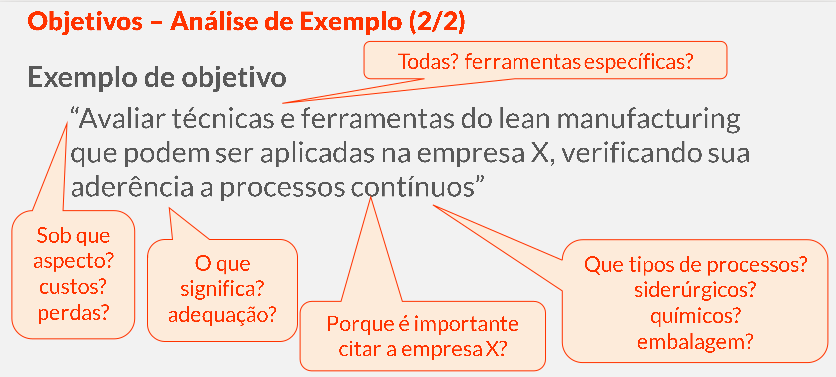
\includegraphics[width=\textwidth]{EstruturaI/objetivo-verbos}
    \end{center}
  \end{exampleblock}

  \vfill
  \scriptsize
  Fonte: VEduca
\end{frame}

\subsection{Métodos}

\subsubsection{Metodologia}

\begin{frame}{Metodologia}
  \footnotesize
  Os métodos são importantes para
  \bigskip
  \begin{itemize}
    \footnotesize
  \item organizar o trabalho acadêmico
    \bigskip
  \item possibilitar a replicação dos resultados
    \bigskip
  \item detalhar os procedimentos, instrumentos e análises utilizadas
  \end{itemize}

  \vfill
  \scriptsize
  Adaptado de: VEduca
\end{frame}

\begin{frame}{Metodologia}
  \footnotesize
  Assim, os métodos visam:
  \bigskip
  \begin{itemize}
    \footnotesize
  \item identificar como os objetivos específicos serão cumpridos
    \bigskip
  \item permitir a leitura crítica do trabalho
    \bigskip
  \item classificar o tipo de trabalho
  \end{itemize}
\end{frame}

\begin{frame}{Metodologia}
  \begin{block}{Importante}
    \footnotesize
    Idealmente, todas as escolhas metodológicas devem ser
    justificadas, seja textualmente, ou por referências.
  \end{block}
\end{frame}

\subsubsection{Tipos de metodologia}

\begin{frame}{Tipos de metodologia}
  \begin{itemize}
    \footnotesize
  \item<1-> Teórico-conceitual
  \bigskip
  \item<1-> Experimental
  \bigskip
  \item<1-> Estudo de caso
  \bigskip
  \item<1-> Pesquisa-ação
  \end{itemize}

  \vfill
  \scriptsize
  Adaptado de: VEduca
\end{frame}

\begin{frame}{Trabalho teórico-conceitual}
  \begin{itemize}
    \footnotesize
  \item Extensão ou refinamento da teoria existente
  \item Nova teoria
  \item Revisão bibliográfica
  \end{itemize}
  \begin{exampleblock}{Exemplo}
    \scriptsize
    Simulação de fenômenos, ou de experimentos. Modelo matemático ou físico.
  \end{exampleblock}

  \vfill
  \scriptsize
  Adaptado de: VEduca
\end{frame}

\begin{frame}{Trabalho experimental}
  \begin{itemize}
    \footnotesize
  \item Investigar uma ou mais relações causais entre variáveis
  \item Condições controladas (laboratório)
  \end{itemize}
  \begin{exampleblock}{Exemplo}
    \scriptsize
    Eficácia de uma nova droga em modelos animais
  \end{exampleblock}

  \vfill
  \scriptsize
  Adaptado de: VEduca
\end{frame}

\begin{frame}{Estudo de caso}
  \begin{itemize}
    \footnotesize
  \item Analisar um fenômeno em um caso concreto
  \item Objeto de análise é específico
  \item Amostra pequena (não raro, $n=1$)
  \item Não pretende generalizar os resultados
  \end{itemize}
  \begin{exampleblock}{Exemplo}
    \scriptsize
    Análise da qualidade de atendimento em um ambulatório (específico).
  \end{exampleblock}

  \vfill
  \scriptsize
  Adaptado de: VEduca
\end{frame}

\begin{frame}{Pesquisa-ação}
  \begin{itemize}
    \footnotesize
  \item Propor uma \alert{intervenção}
  \item Variante do estudo de caso
  \item Pesquisador interfere no objeto de estudo
  \end{itemize}
  \begin{exampleblock}{Exemplo}
    \scriptsize
    Identificação (e possivelmente resolução) de problema no
    atendimento de um ambulatório específico, visando reduzir o tempo
    de espera.
  \end{exampleblock}

  \vfill
  \scriptsize
  Fontes: VEduca, Koerich {\em et al}, 2009.
\end{frame}

\begin{frame}{Pesquisa-ação}
  \begin{center}
    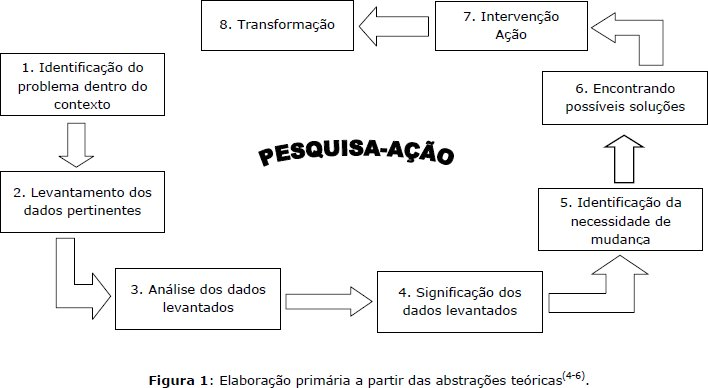
\includegraphics[width=\textwidth]{EstruturaI/pesquisa-acao}
  \end{center}

  \vfill
  \scriptsize
  Fonte: Koerich {\em et al}, 2009.
\end{frame}

\subsection{Resultados}

\subsubsection{Resultados esperados}

\begin{frame}{Resultados esperados}
  \begin{itemize}
    \footnotesize
  \item Confirmação ou refutação das hipóteses descritas
  \bigskip
  \item Inferência de causalidade entre variáveis
  \bigskip
  \item Divulgação e publicação de relatório, artigo, congresso,
    dissertação, tese, etc.
  \bigskip
  \item Obtenção de titulação {\em stricto sensu} ou {\em lato sensu}
  \end{itemize}
\end{frame}

\subsubsection{Resultados preliminares}

\begin{frame}{Resultados preliminares}
  \scriptsize
  Caso disponíveis, resultados preliminares devem ser descritos para:
  \bigskip
  \begin{itemize}
    \footnotesize
  \item Validar a metodologia
  \bigskip
  \item Indicar o rumo da pesquisa (qualidade)
  \bigskip
  \item Testar (preliminarmente) a análise:
    \begin{itemize}
      \scriptsize
    \item dos dados
    \item das hipóteses
    \end{itemize}
  \bigskip
  \item Transmitir confiança aos avaliadores (prazo)
  \end{itemize}
\end{frame}

\begin{frame}{Resultados preliminares}
  \scriptsize
  Podem ser descritos:
  \bigskip
  \begin{itemize}
    \footnotesize
  \item Em uma coleta preliminar, em pequena escala (piloto)
  \bigskip
  \item Em um estágio inicial da coleta
  \bigskip
  \item Após a coleta completa, mas análise de um subconjunto dos dados
  \end{itemize}
\end{frame}

\subsection{Introdução}

\begin{frame}{Introdução}
  \begin{itemize}
    \footnotesize
  \item Situa o trabalho em um contexto acadêmico
  \bigskip
  \item Justifica a importância do problema de pesquisa
  \bigskip
  \item Relevância do trabalho
  \bigskip
  \item Mapeia a estrutura do texto
  \bigskip
  \item Se separado da Revisão bibliográfica, pequena \footnote{o
      contexto será detalhado na Revisão}
  \end{itemize}
\end{frame}

\begin{frame}{Obrigatório}
  \scriptsize
  A introdução deve incluir:
  \bigskip
  \begin{itemize}
    \footnotesize
  \item O tema e a justificativa
  \bigskip
  \item A relevância e as contribuições para a área
  \bigskip
  \item O problema de pesquisa
  \bigskip
  \item A hipótese estabelecida
  \bigskip
  \item Os objetivos\footnote{Em muitas instituições, estes estão em capítulo próprio}
  \end{itemize}

  \vfill
  \scriptsize
  Fonte: Prodanov, 2013
\end{frame}

\begin{frame}{Exemplo (mapeando um trabalho longo)}
  \begin{exampleblock}{Exemplo (fechamento da Introdução)}
    \begin{center}
      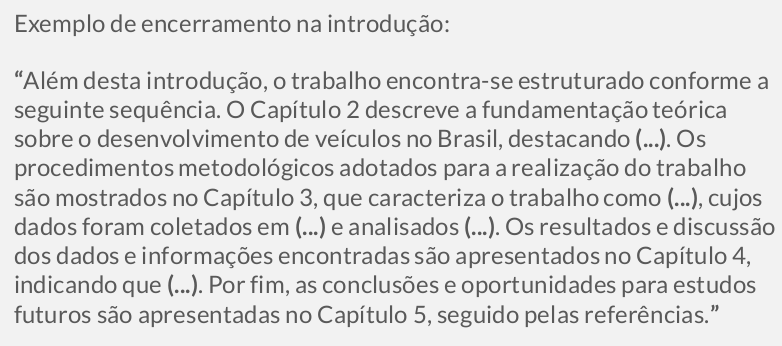
\includegraphics[width=\textwidth]{EstruturaI/exemplo-introducao}
    \end{center}
  \end{exampleblock}

  \vfill
  \scriptsize
  Fonte: VEduca
\end{frame}

\begin{frame}{Introdução $\times$ Revisão}
  \begin{itemize}
    \footnotesize
  \item Organização do projeto depende da Instituição
  \bigskip
  \item Por vezes, a Introdução (seção ou capítulo) inclui:
    \begin{itemize}
      \scriptsize
    \item Contexto, Justificativa
    \item Revisão
    \item Objetivos
    \end{itemize}
  \bigskip
  \item Outras vezes, cada uma dessas seções é apresentada em capítulo
    separado
  \bigskip
  \item É importante \alert{consultar} a norma \alert{específica} a
    ser atendida
  \end{itemize}
\end{frame}

\section{Aprofundamento}

\subsection{Aprofundamento}

\begin{frame}{Aprofundamento}
  \begin{block}{Leitura obrigatória}
    \scriptsize
    Seções do livro texto:
    \begin{itemize}
      \scriptsize
    \item {\bf Objetivos} 4.5
    \item {\bf Métodos} 4.6
    % \item {\bf Resultados}
    \item {\bf Introdução} 4.1 -- 4.4
    \end{itemize}
  \end{block}
  \begin{block}{Leitura recomendada}
    \begin{itemize}
      \scriptsize
    \item<1-> \href{http://www.veduca.com.br/assistir/metodologia-cientifica}
      {VEduca: video aulas}
    \item<1-> \href{http://www.veduca.com.br/assistir/metodologia-cientifica}
      {Koerich et al (2009): Pesquisa-ação: ferramenta
      metodológica para a pesquisa qualitativa (Rev. Eletr. Enf.)}
  \item<1-> \href{http://www.veduca.com.br/assistir/metodologia-cientifica}
    {Estrutura de um projeto e Técnicas de Leitura (Youtube)}
      % \item<1-> Prodanov (2013): cap 4.
      % \item<1-> Lakatos (2003): cap 10.
    \end{itemize}
  \end{block}
\end{frame}

\end{document}
